\documentclass{homework}

\input{particulars}

\sisetup{round-precision=3}

\begin{document}

\title{Video Compression HW3}
\author{\chineseName \masterStudentID}
\date{}
\maketitle

% \begin{figure}[H]
%     \centering
%     \begin{subfigure}{0.32\textwidth}
%         \centering
%         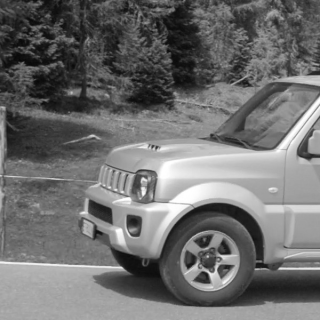
\includegraphics[width=0.9\textwidth]{one_gray.png}
%         \caption{one\_gray.png}
%     \end{subfigure}
%     \begin{subfigure}{0.32\textwidth}
%         \centering
%         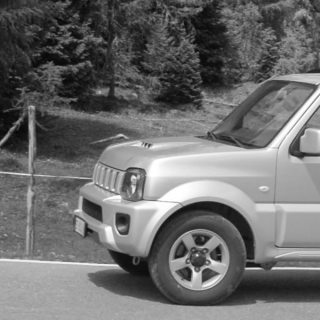
\includegraphics[width=0.9\textwidth]{two_gray.png}
%         \caption{two\_gray.png}
%     \end{subfigure}
%     \caption{Original frames}
% \end{figure}

\section*{Full Search Motion Estimation}

\begin{figure}[H]
    \centering
    \begin{subfigure}{0.32\textwidth}
        \centering
        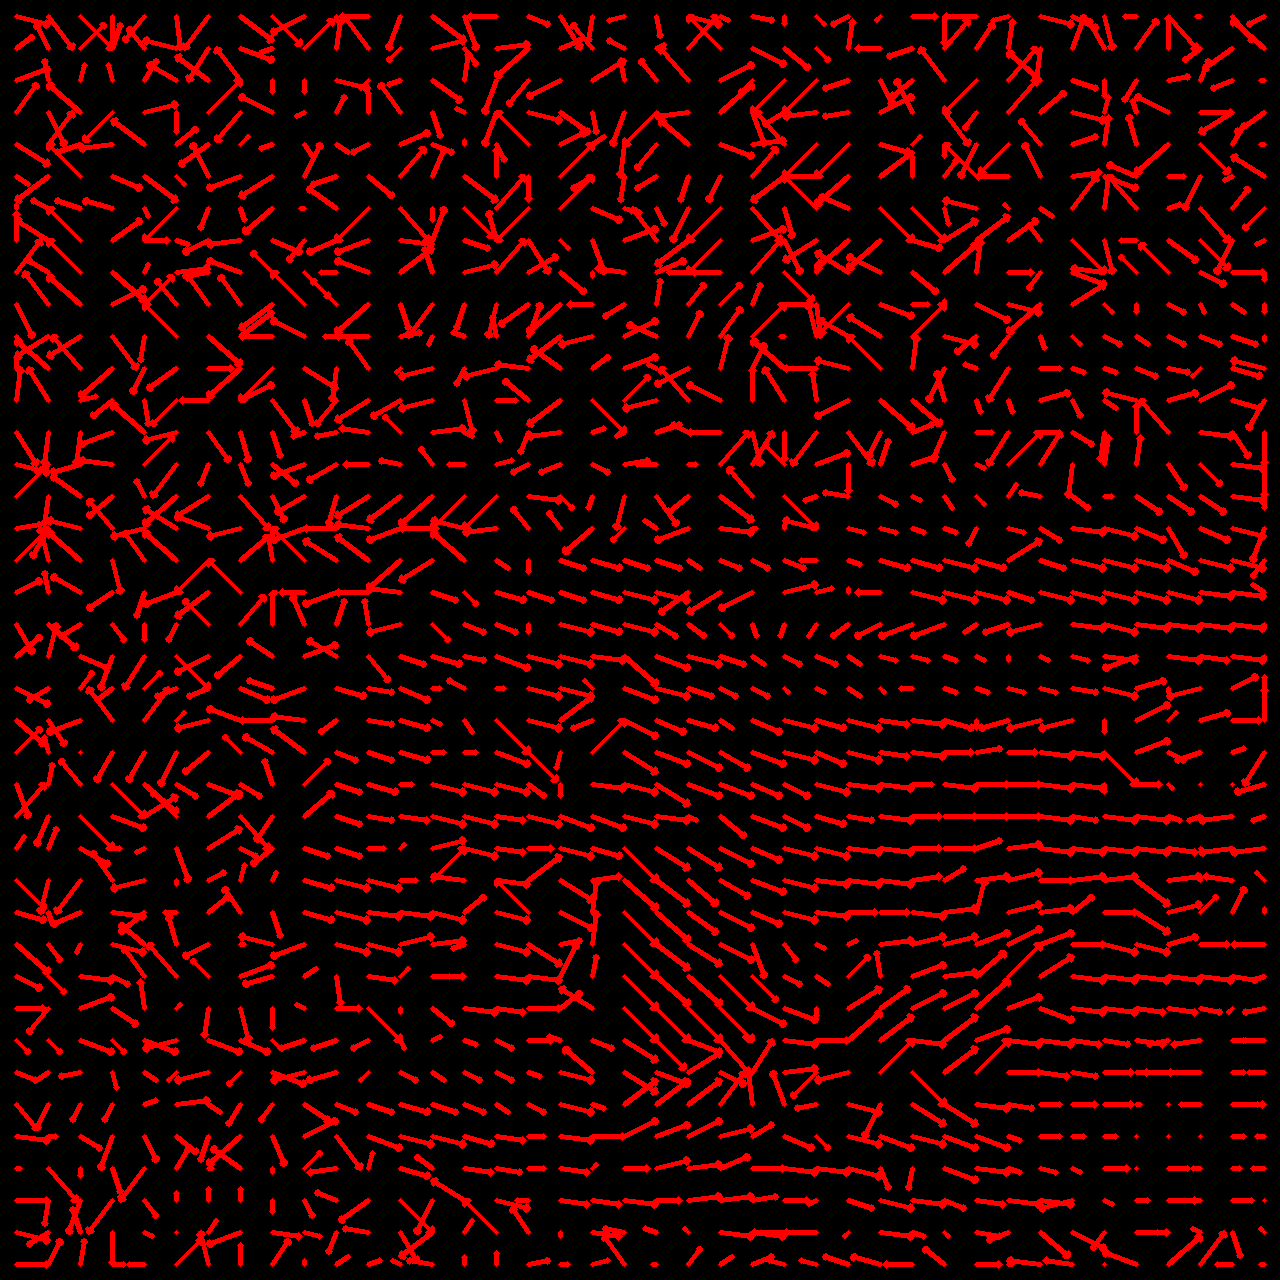
\includegraphics[width=0.9\textwidth]{8_8_motion_vectors.png}
        \caption{Motion vectors}
    \end{subfigure}
    \begin{subfigure}{0.32\textwidth}
        \centering
        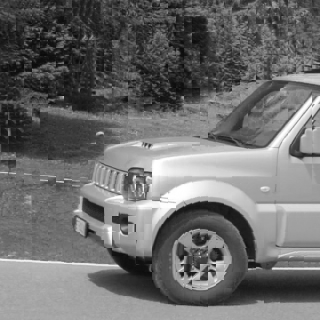
\includegraphics[width=0.9\textwidth]{8_8_motion_compensation.png}
        \caption{Reconstructed frame}
    \end{subfigure}
    \begin{subfigure}{0.32\textwidth}
        \centering
        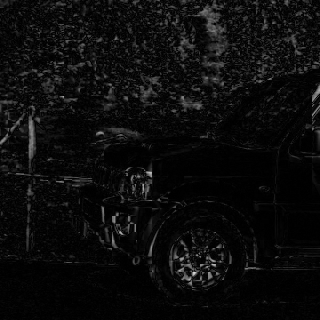
\includegraphics[width=0.9\textwidth]{8_8_residual.png}
        \caption{Residual}
    \end{subfigure}
    \caption{search range = $[\pm 8]$}
\end{figure}

\begin{figure}[H]
    \centering
    \begin{subfigure}{0.32\textwidth}
        \centering
        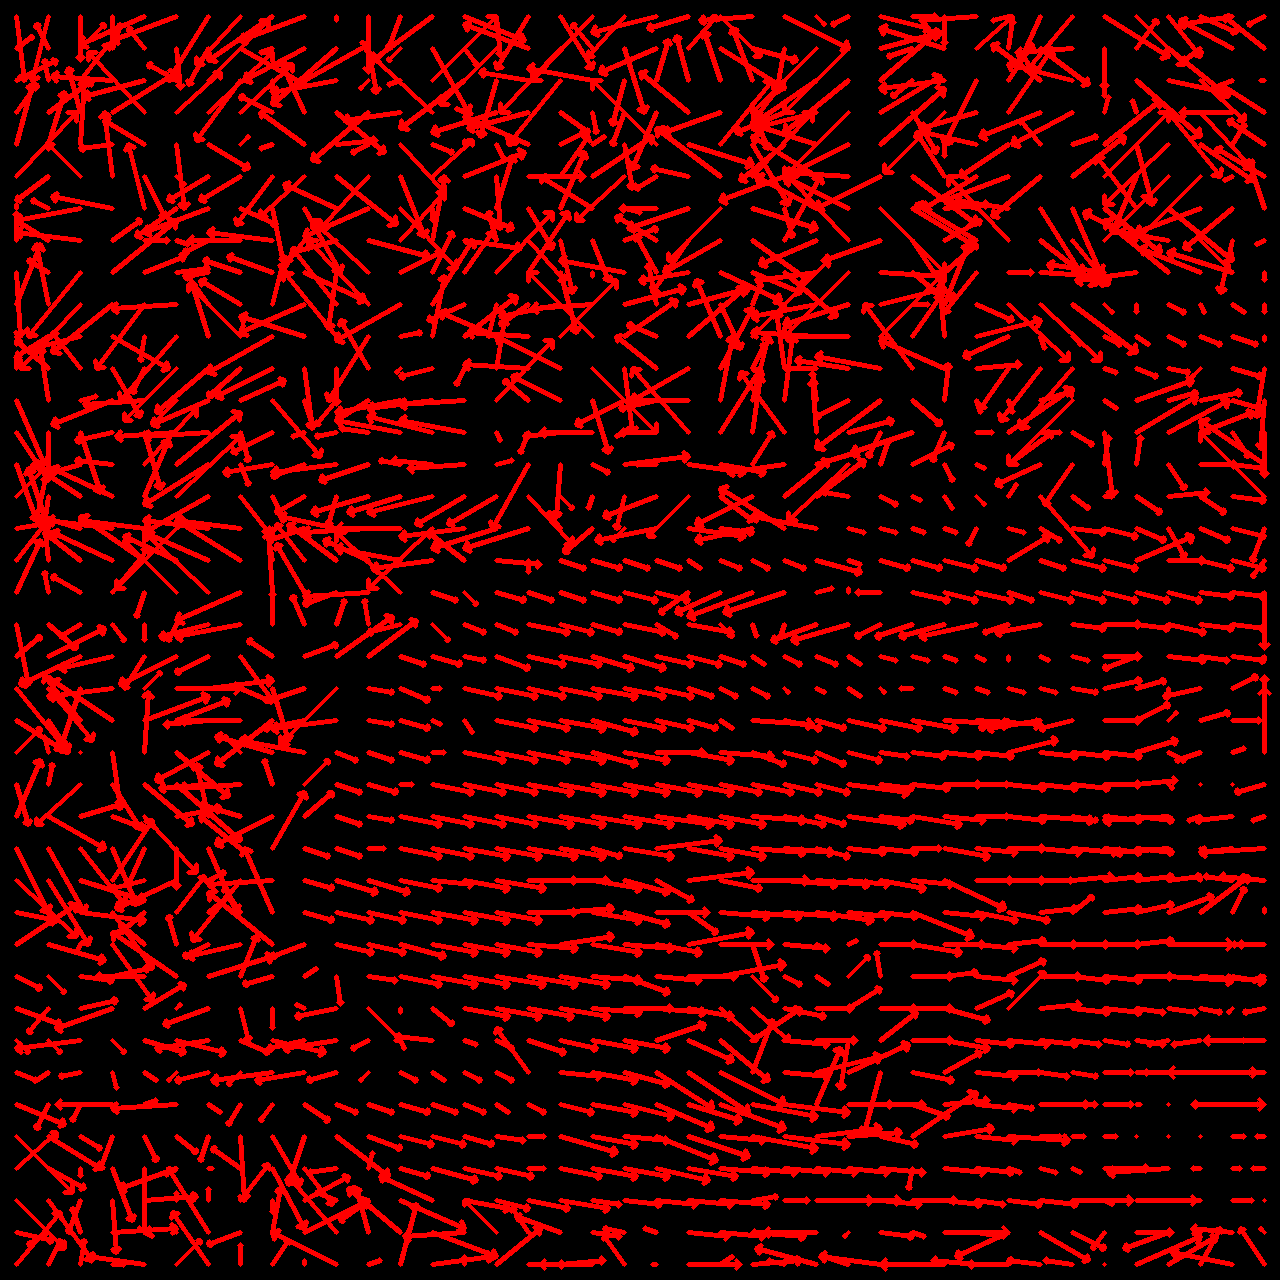
\includegraphics[width=0.9\textwidth]{8_16_motion_vectors.png}
        \caption{Motion vectors}
    \end{subfigure}
    \begin{subfigure}{0.32\textwidth}
        \centering
        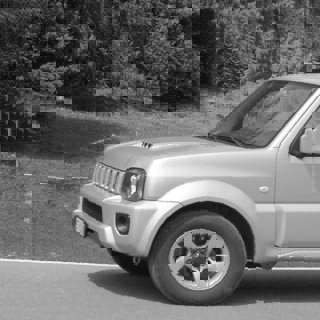
\includegraphics[width=0.9\textwidth]{8_16_motion_compensation.png}
        \caption{Reconstructed frame}
    \end{subfigure}
    \begin{subfigure}{0.32\textwidth}
        \centering
        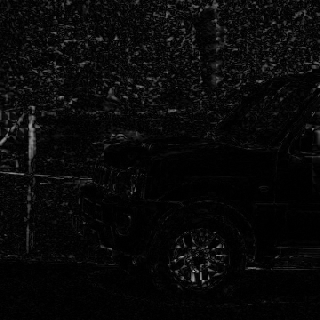
\includegraphics[width=0.9\textwidth]{8_16_residual.png}
        \caption{Residual}
    \end{subfigure}
    \caption{search range = $[\pm 16]$}
\end{figure}

\begin{figure}[H]
    \centering
    \begin{subfigure}{0.32\textwidth}
        \centering
        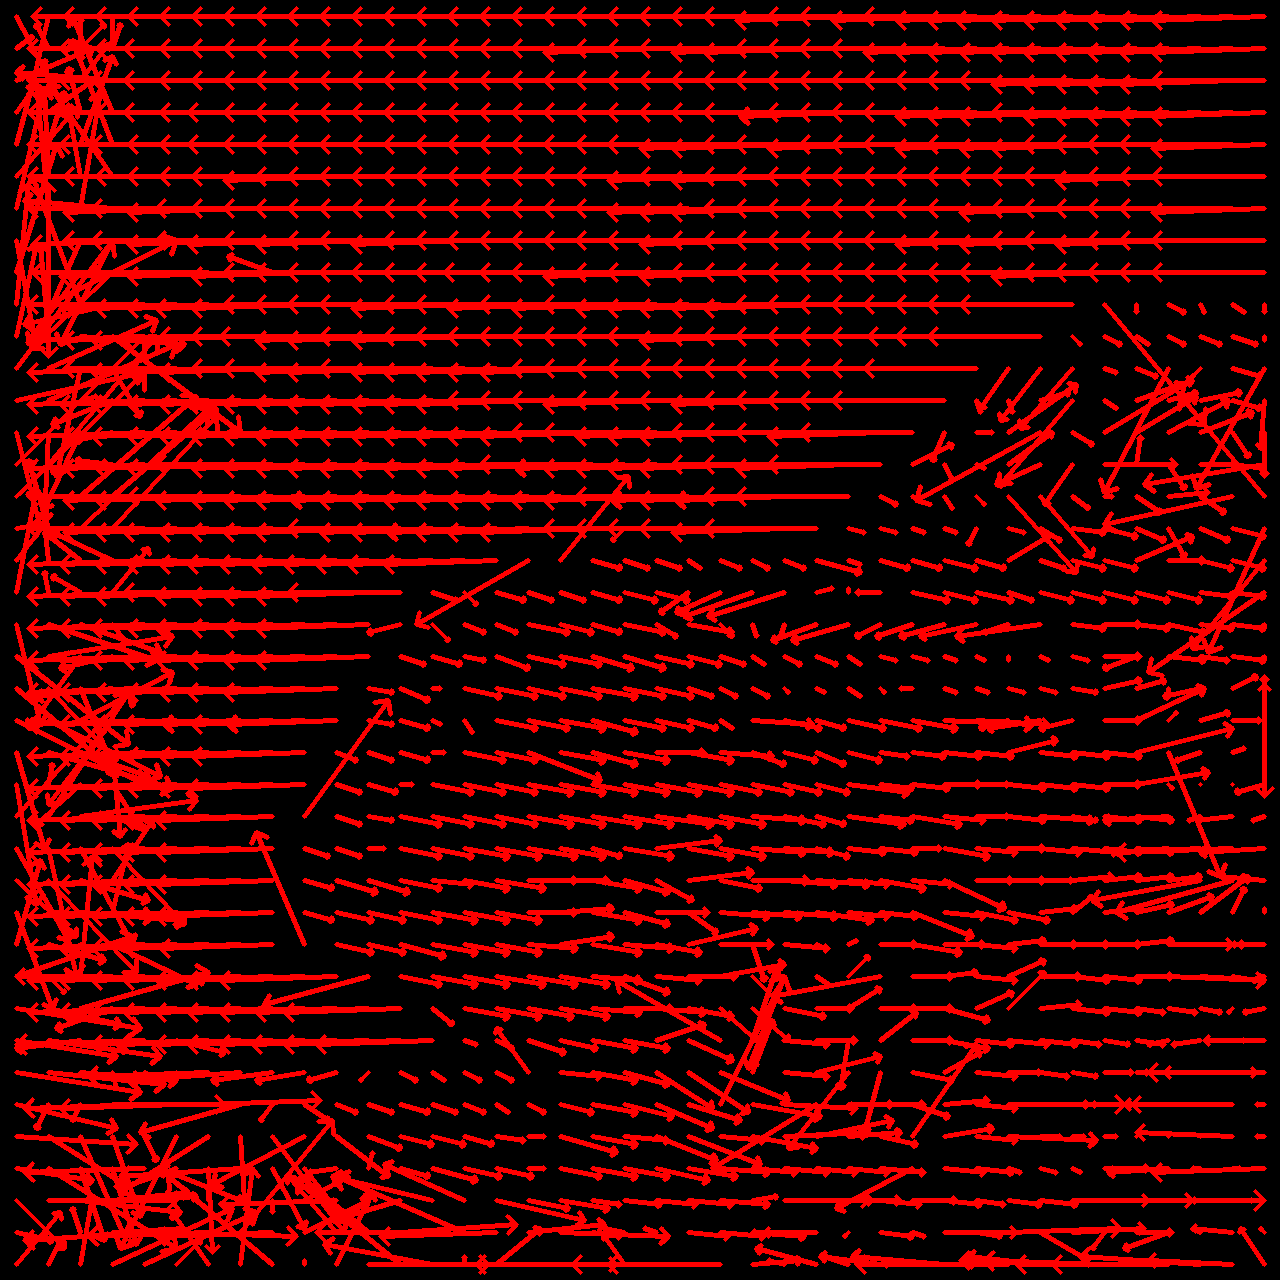
\includegraphics[width=0.9\textwidth]{8_32_motion_vectors.png}
        \caption{Motion vectors}
    \end{subfigure}
    \begin{subfigure}{0.32\textwidth}
        \centering
        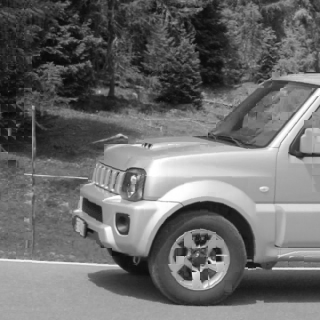
\includegraphics[width=0.9\textwidth]{8_32_motion_compensation.png}
        \caption{Reconstructed frame}
    \end{subfigure}
    \begin{subfigure}{0.32\textwidth}
        \centering
        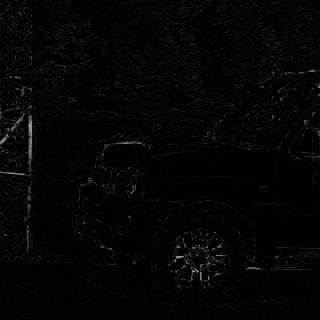
\includegraphics[width=0.9\textwidth]{8_32_residual.png}
        \caption{Residual}
    \end{subfigure}
    \caption{search range = $[\pm 32]$}
\end{figure}

\section*{Three Step Search Motion Estimation}

\begin{figure}[H]
    \centering
    \begin{subfigure}{0.32\textwidth}
        \centering
        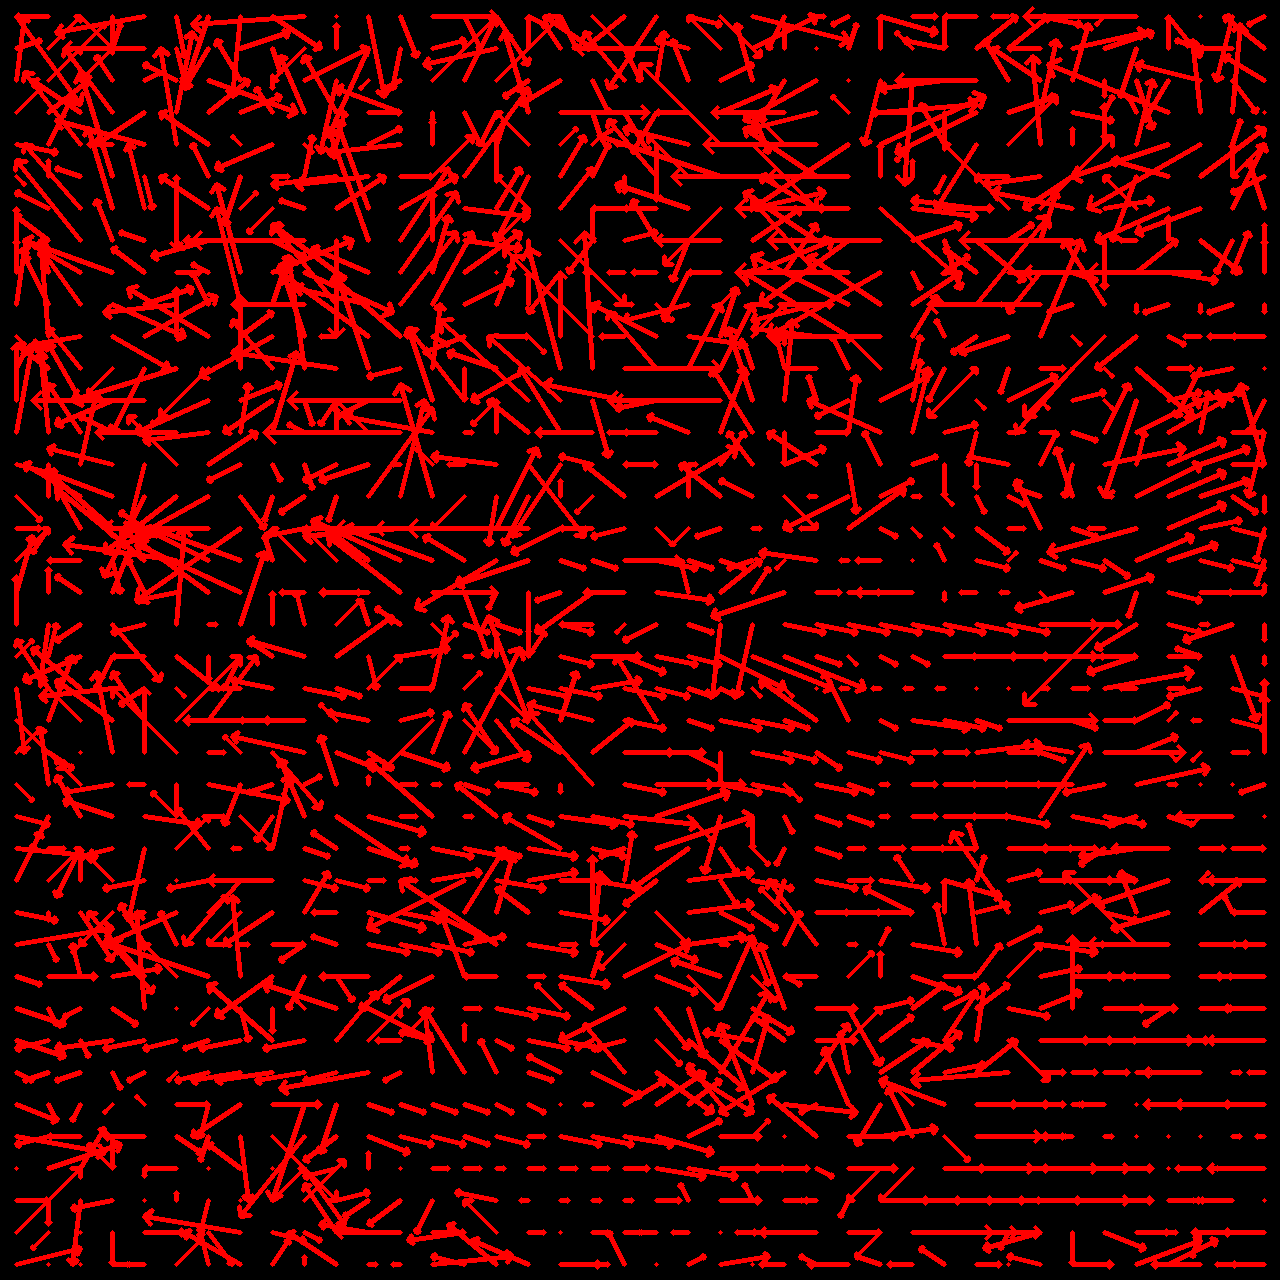
\includegraphics[width=0.9\textwidth]{8_8_TSS_motion_vectors.png}
        \caption{Motion vectors}
    \end{subfigure}
    \begin{subfigure}{0.32\textwidth}
        \centering
        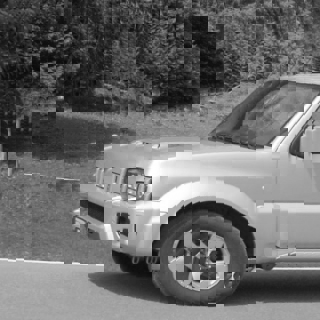
\includegraphics[width=0.9\textwidth]{8_8_TSS_motion_compensation.png}
        \caption{Reconstructed frame}
    \end{subfigure}
    \begin{subfigure}{0.32\textwidth}
        \centering
        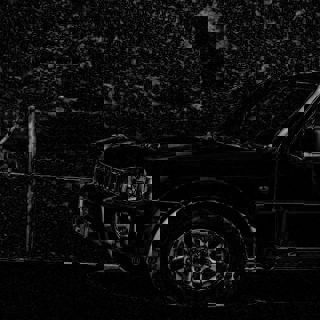
\includegraphics[width=0.9\textwidth]{8_8_TSS_residual.png}
        \caption{Residual}
    \end{subfigure}
    \caption{search range = $[\pm 8]$}
\end{figure}

\begin{figure}[H]
    \centering
    \begin{subfigure}{0.32\textwidth}
        \centering
        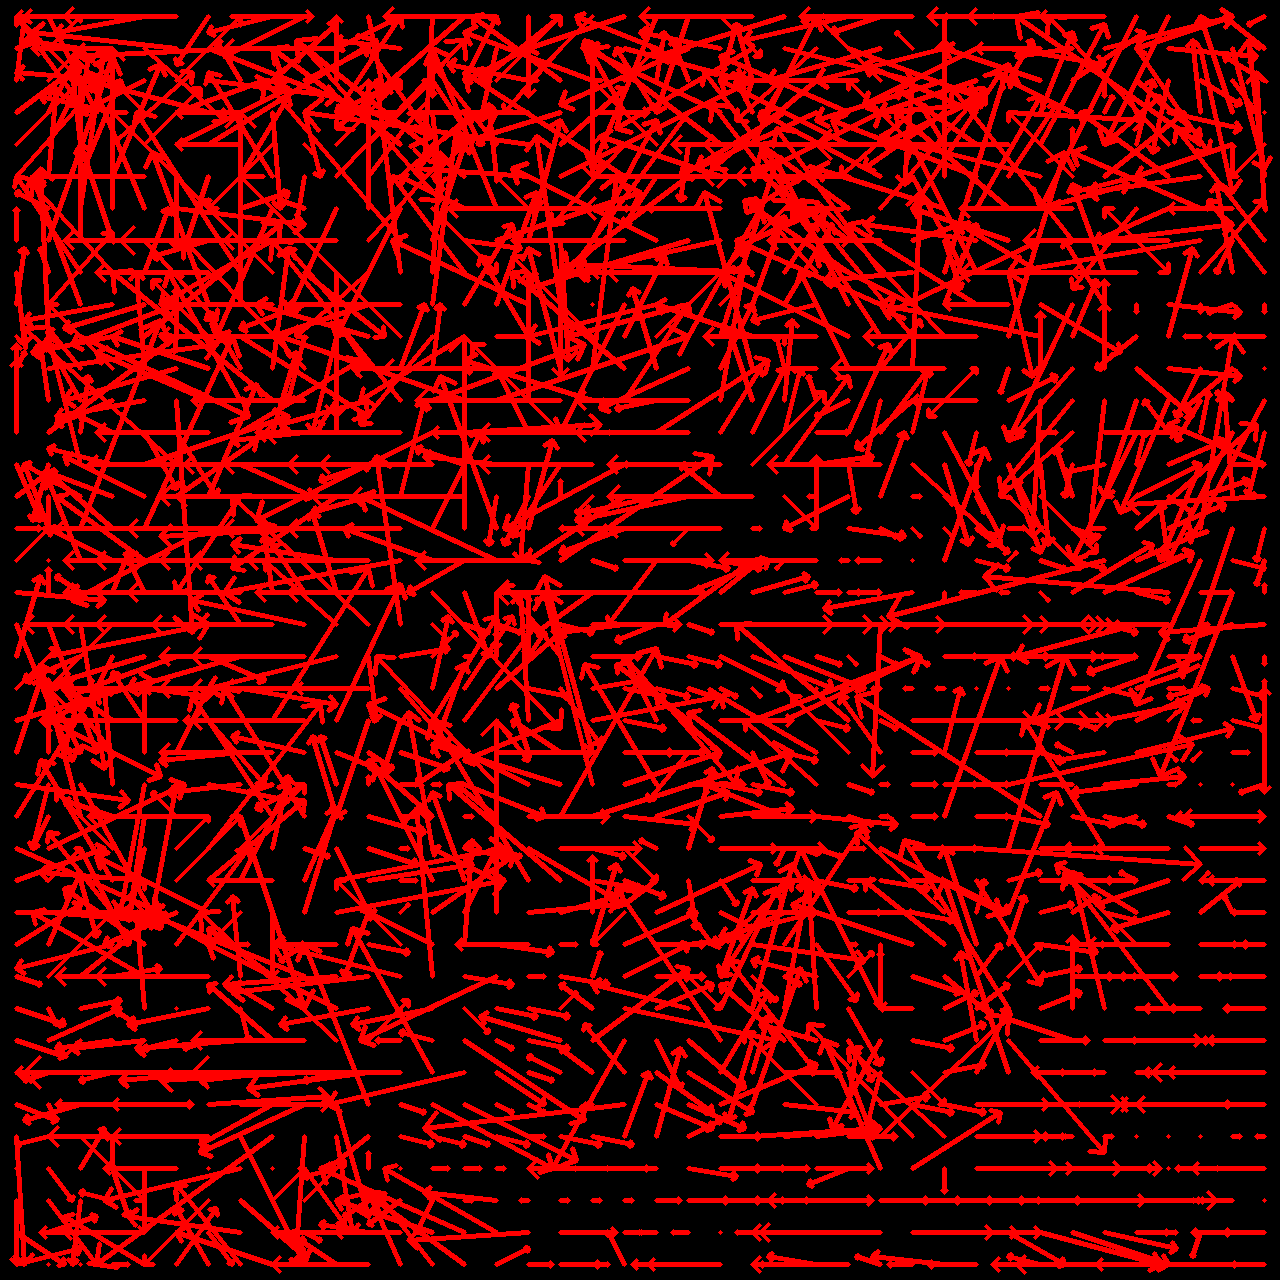
\includegraphics[width=0.9\textwidth]{8_16_TSS_motion_vectors.png}
        \caption{Motion vectors}
    \end{subfigure}
    \begin{subfigure}{0.32\textwidth}
        \centering
        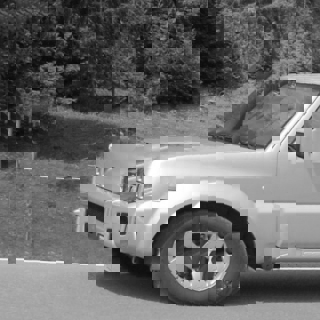
\includegraphics[width=0.9\textwidth]{8_16_TSS_motion_compensation.png}
        \caption{Reconstructed frame}
    \end{subfigure}
    \begin{subfigure}{0.32\textwidth}
        \centering
        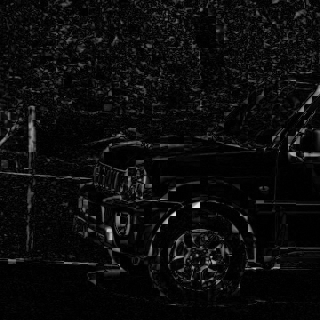
\includegraphics[width=0.9\textwidth]{8_16_TSS_residual.png}
        \caption{Residual}
    \end{subfigure}
    \caption{search range = $[\pm 16]$}
\end{figure}

\begin{figure}[H]
    \centering
    \begin{subfigure}{0.32\textwidth}
        \centering
        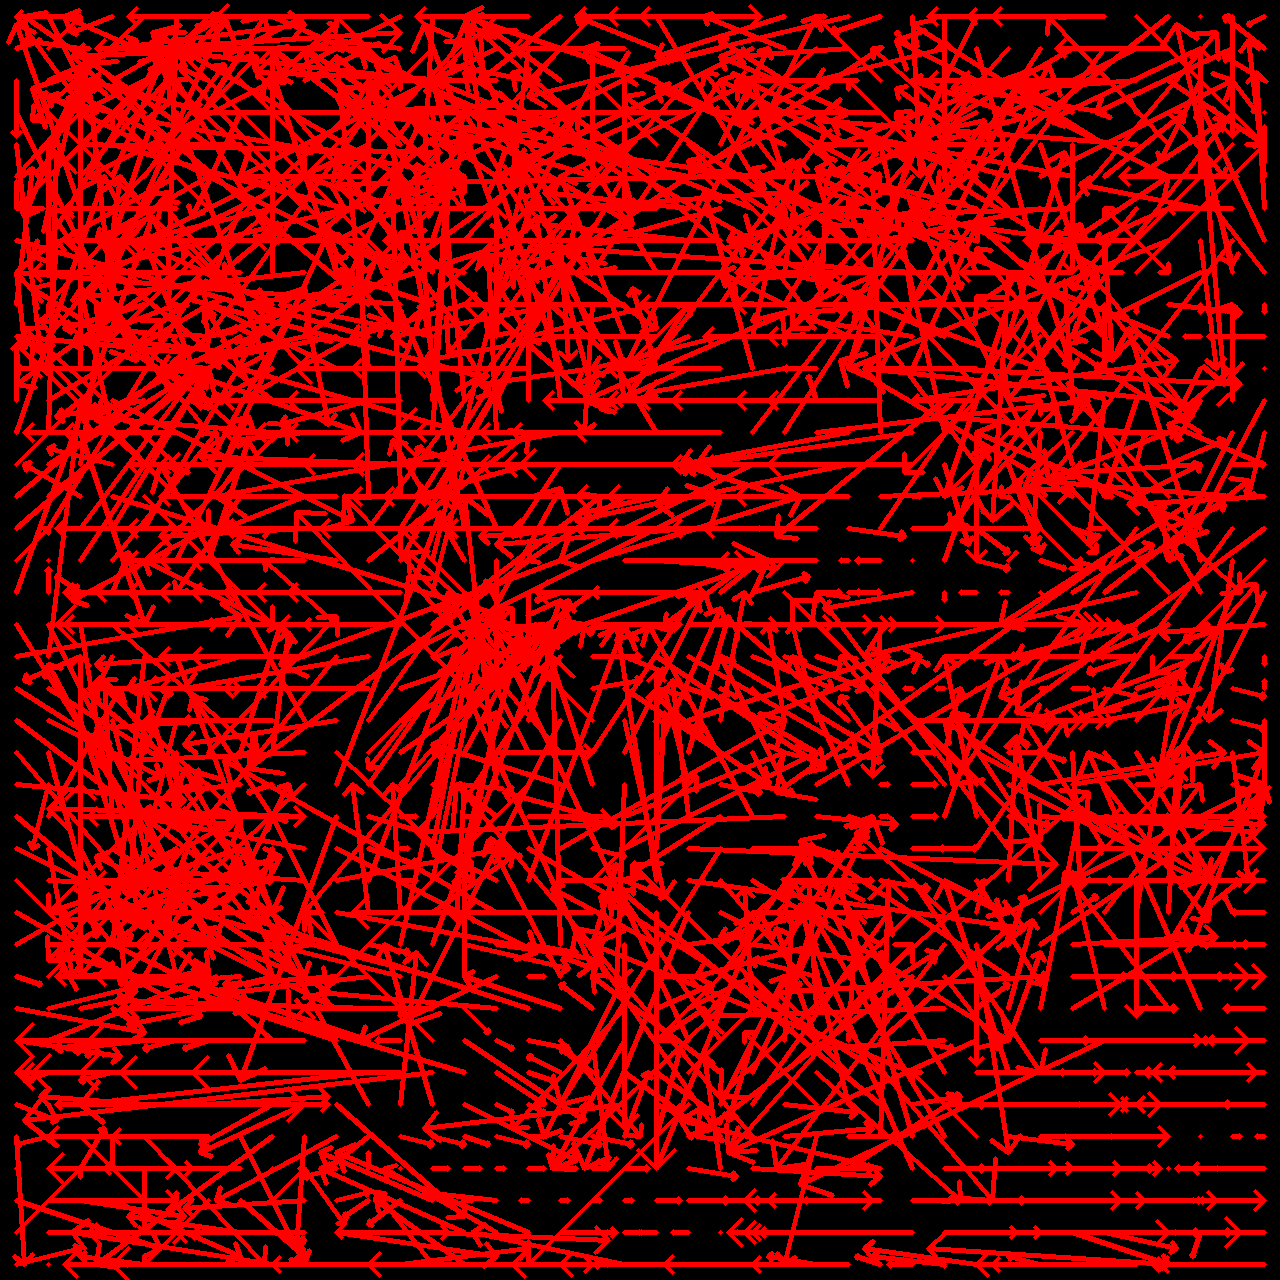
\includegraphics[width=0.9\textwidth]{8_32_TSS_motion_vectors.png}
        \caption{Motion vectors}
    \end{subfigure}
    \begin{subfigure}{0.32\textwidth}
        \centering
        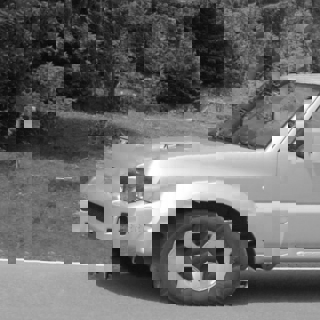
\includegraphics[width=0.9\textwidth]{8_32_TSS_motion_compensation.png}
        \caption{Reconstructed frame}
    \end{subfigure}
    \begin{subfigure}{0.32\textwidth}
        \centering
        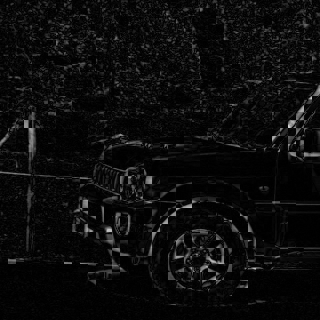
\includegraphics[width=0.9\textwidth]{8_32_TSS_residual.png}
        \caption{Residual}
    \end{subfigure}
    \caption{search range = $[\pm 32]$}
\end{figure}

The PSNR and runtime are reported as follows.

% Full search
% Block size: 8
% Search range: 8
% PSNR: 28.8956
% Execution time: 0.446452 s
% Block size: 8
% Search range: 16
% PSNR: 29.9308
% Execution time: 1.59561 s
% Block size: 8
% Search range: 32
% PSNR: 32.3672
% Execution time: 5.6676 s

% Three step search
% Block size: 8
% Search range: 8
% PSNR: 28.618
% Execution time: 0.0609975 s
% Block size: 8
% Search range: 16
% PSNR: 28.8256
% Execution time: 0.0723592 s
% Block size: 8
% Search range: 32
% PSNR: 28.8845
% Execution time: 0.0897082 s

\begin{table}[H]
    \centering
    \begin{tabular}{|c|c|c|c|c|}
        \hline
        Method & Block Size & Search Range & PSNR (dB) & Execution Time (s) \\
        \hline
        & 8 & 8 & \num{28.8956} & \num{0.446452} \\
        Full Search & 8 & 16 & \num{29.9308} & \num{1.59561} \\
        & 8 & 32 & \num{32.3672} & \num{5.6676} \\
        \hline
        & 8 & 8 & \num{28.618} & \num{0.0609975} \\
        Three Step Search & 8 & 16 & \num{28.8256} & \num{0.0723592} \\
        & 8 & 32 & \num{28.8845} & \num{0.0897082} \\
        \hline
    \end{tabular}
    \caption{PSNR and Execution Time for Different Block Sizes and Search Ranges}
\end{table}

\end{document}